\apendice{Especificación de Requisitos}

\section{Introducción}

\section{Objetivos generales}
El desarrollo del proyecto busca lograr los siguientes objetivos:
\begin{itemize}
\item
Desarrollar un fichero de diseño del juego que resuma en qué va a consistir el juego y que mecánicas implementará.
\item
Desarrollar un videojuego que implemente las mecánicas definidas en el fichero de diseño del juego.
\item
Ofrecer versiones del producto final (el videojuego) para Windows, Linux y WebGL.
\item
Ofrecer un juego controlable tanto con teclado y ratón como con mando.
\end{itemize}

\section{Catalogo de requisitos}
\subsection{Requisitos funcionales}
Los requisitos funcionales especificarán cual es el funcionamiento que se espera del producto. Se concretarán a continuación.

\begin{itemize}
\item
\textbf{RF-1 Gestión de menús:}El jugador deber poder navegar por los menús.

\begin{itemize}
\item
\textbf{RF-1.1 Navegación entre pantallas:} Las pantallas deben de permitir navegar a otras pantallas (de manera directa o indirecta).
\end{itemize}

\item
\textbf{RF-2 Gestión del menú principal:} Deberá haber un menú principal que sea la primera escena que se muestre en el videojuego.

\begin{itemize}
\item
\textbf{RF-2.1 Selección de nivel:} Debe de poderse acceder a cualquier nivel desde el menú principal.
\end{itemize}

\begin{itemize}
\item
\textbf{RF-2.2 Cierre de la aplicación:} Se debe de poder cerrar la aplicación desde el menú principal.
\end{itemize}

\begin{itemize}
\item
\textbf{RF-2.3 Viaje al menú de opciones:} Se puede viajar desde el menú principal al menú de opciones.
\end{itemize}

\item
\textbf{RF-3 Gestión del menú de opciones:} Deberá haber un menú de opciones que permita modificar aspectos generales del juego. Desde el menú de opciones se debe poder volver al menú principal.

\item
\textbf{RF-4 Gestión de niveles:} Los niveles deben de contener todos los elementos necesarios y obligatorios de un nivel.

\begin{itemize}
\item
\textbf{RF-4.1 Controlar un avatar:} Debe de haber un avatar controlable por el jugador que realice las operaciones que le indique el jugador.
\end{itemize}

\begin{itemize}
\item
\textbf{RF-4.2 Zonas de muerte:} Debe haber zonas que maten al avatar del jugador cuando entre en contacto con ellas y devuelvan el nivel a un estado inicial.
\end{itemize}

\begin{itemize}
\item
\textbf{RF-4.3 Zonas de victoria (meta):} Debe haber zonas en las que, al entrar, se considere el nivel terminado y se vuelva al menú principal.
\end{itemize}

\begin{itemize}
\item
\textbf{RF-4.4 Gestión del menú de pausa:} Se debe poder acceder al menú de pausa, que parará la ejecución del nivel.

\begin{itemize}
\item
\textbf{RF-4.4.1 Abrir el menú de pausa:} Se deberá de poder abrir el menú de pausa, lo que pausara la ejecución del nivel.
\end{itemize}

\begin{itemize}
\item
\textbf{RF-4.4.2 Operaciones del menú de pausa:} Se deben de poder realizar las mismas operaciones que en el menú de opciones.
\end{itemize}

\begin{itemize}
\item
\textbf{RF-4.4.3 Cerrar el menú de pausa:} Se deberá poder cerrar el menú de pausa, lo que reanudará la ejecución del nivel.
\end{itemize}
\end{itemize}

\begin{itemize}
\item
\textbf{RF-4.5 Manipulación de la gravedad:} Debe de ser posible manipular la gravedad del nivel.
\end{itemize}

\begin{itemize}
\item
\textbf{RF-4.6 Manipulación del tiempo:} Debe de ser posible modificar la escala de tiempo que afecta al nivel.
\end{itemize}

\begin{itemize}
\item
\textbf{RF-4.7 Aplicación de impulsos:} Se debe poder aplicar impulsos que varíen la trayectoria que lleva un objeto.
\end{itemize}

\begin{itemize}
\item
\textbf{RF-4.8 Obstáculos:} Puede haber obstáculos que maten al avatar jugable cuando entre en contacto con ellos.
\end{itemize}

\begin{itemize}
\item
\textbf{RF-4.9 Portales:} Puede haber portales que teletransporten al avatar jugable desde el punto en el que se encuentra a otro que corresponderá con otro portal.
\end{itemize}
\end{itemize}

\begin{itemize}
\item
\textbf{RF-5 Gestión del avatar del jugador:} El jugador debe contar con un avatar controlable por el este. El avatar debe ser capaz de: saltar, moverse, realizar un acelerón y activar el tiempo bala.
\end{itemize}

\subsection{Requisitos no funcionales}
Al ser el producto a entregar un videojuego (un software de ocio), resulta clave especificar que requisitos no funcionales se van a tener en cuenta.

\begin{itemize}
\item
\textbf{Facilidad de uso:} Un videojuego cuyo uso no sea sencillo y cómodo puede perder muchos jugadores por esa única razón. Es clave que los jugadores tengan una experiencia agradable cuando interactúen con el juego.

\item
\textbf{Soporte:} Los cambios y actualizaciones del videojuego tienen que ser trasparentes al usuario, pues no tiene necesidad de conocer como funciona internamente el juego, sino solo abrir el ejecutable y disfrutar del juego.

\item
\textbf{Apariencia o interfaz externa (\textit{look and feel}):} No se ha especificado un diseño de interfaz, sin embargo en el mundo de los videojuegos hay un modelo general muy establecido. Es lógico adoptarlo para ofrecerle al jugador una experiencia que le resulte familiar.

\item
\textbf{Escalabilidad:} En un videojuego se van a ir añadiendo continuamente funcionalidades sobre el código para poder implementar todas las mecánicas, tanto definidas como que puedan surgir en el futuro. Por ello el código debe ser fácil de mantener y extender.
\end{itemize}


\section{Especificación de requisitos}
\subsection{Diagramas de casos de uso}
\begin{figure}[h]
\centering
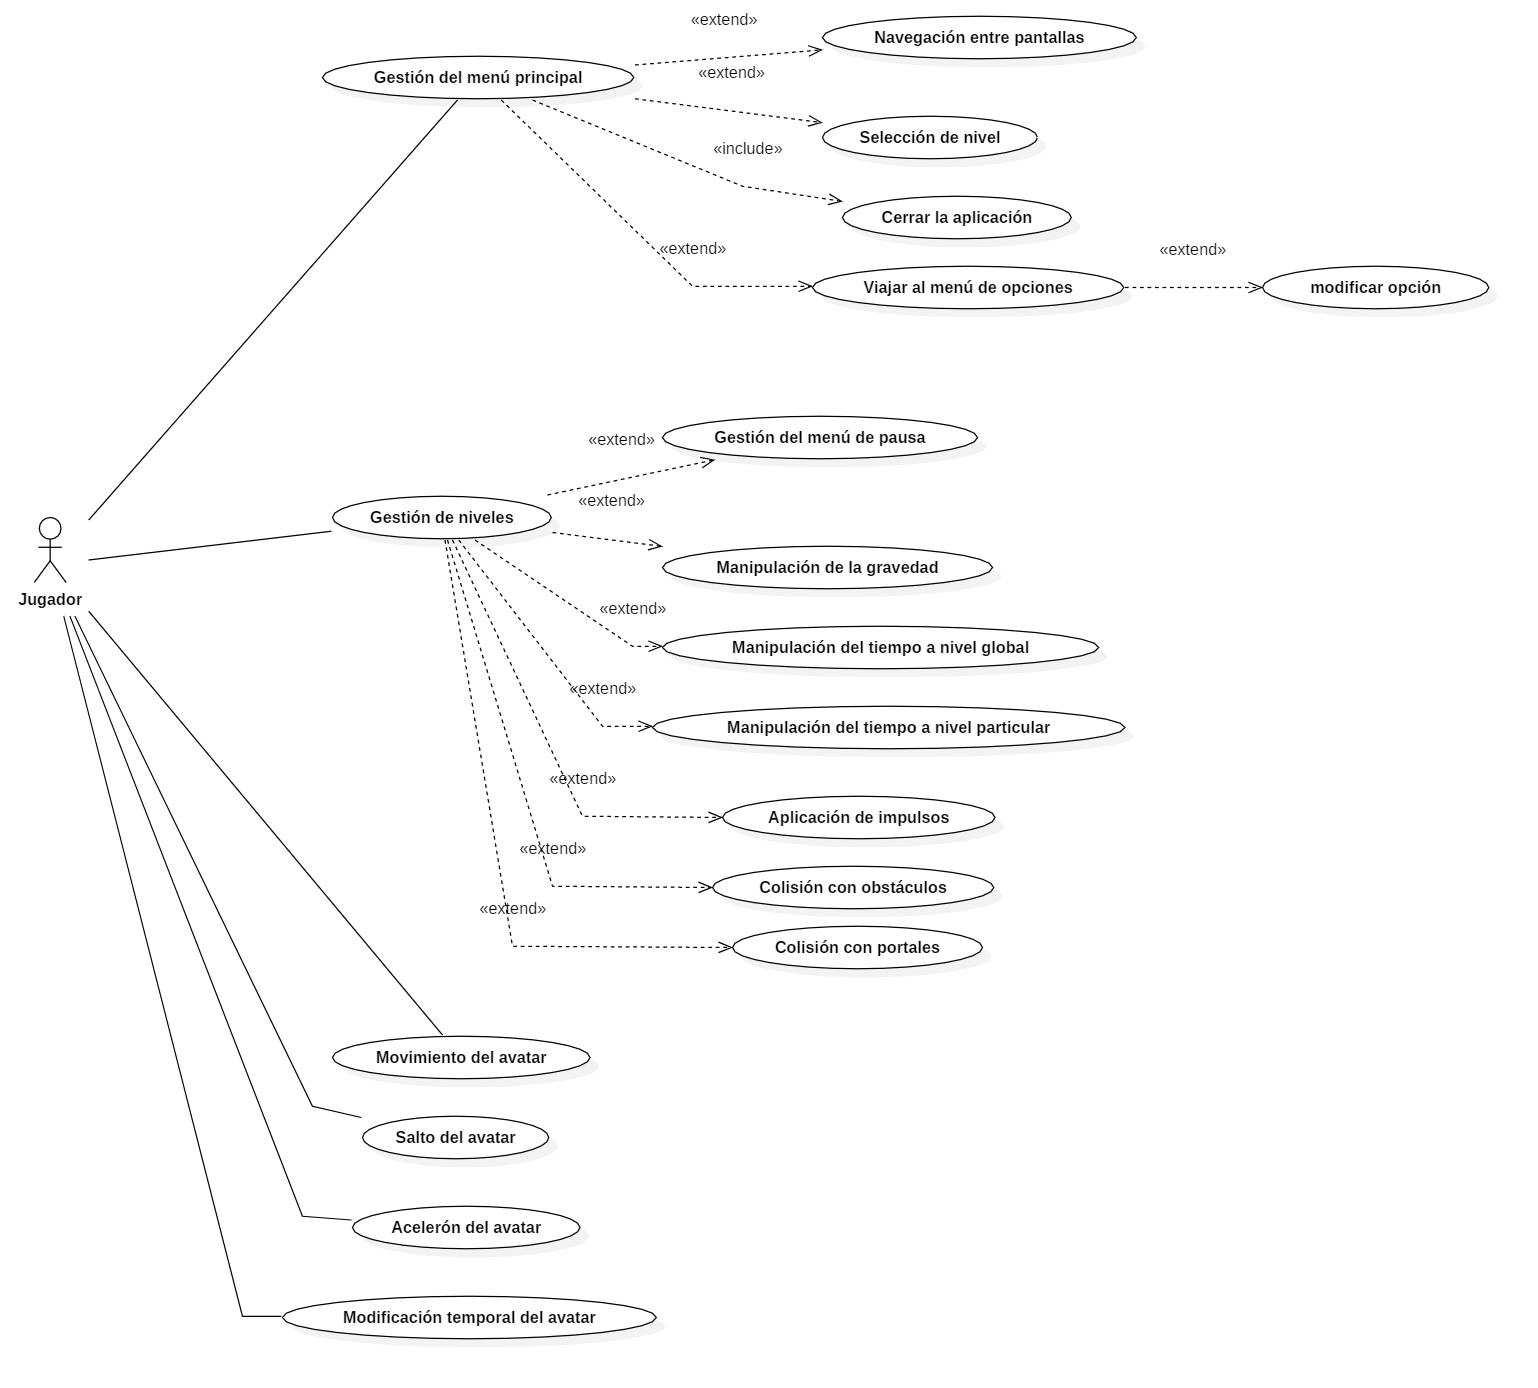
\includegraphics[scale=0.25]{Anexos/Anexo_B/casos_de_uso}
\caption{Diagrama de casos de uso}
\end{figure}

\subsection{Actores}
Solo habrá un actor: el jugador del videojuego.
\subsection{Casos de uso}

\subsubsection{Caso de uso 01}

\begin{longtable}{l|l}
\begin{minipage}{0.25\columnwidth}
\textbf{CU-01} 
\end{minipage}
&
\begin{minipage}{0.65\columnwidth}
Gestión del menú principal
\end{minipage}
\\ \hline

\begin{minipage}{0.25\columnwidth}
\textbf{Descripción} 
\end{minipage}
&
\begin{minipage}{0.65\columnwidth}
Permite al usuario seleccionar escena, cerrar el juego y acceder al menú de opciones
\end{minipage}
\\ \hline

\begin{minipage}{0.25\columnwidth}
\textbf{Requisitos funcionales} 
\end{minipage}
&
\begin{minipage}{0.65\columnwidth}
RF-1, RF-1.1, RF-2, RF-2.1, RF-2.2, RF-2.3                                                                                                                    
\end{minipage}
\\ \hline

\begin{minipage}{0.25\columnwidth}
\textbf{Precondición} 
\end{minipage}
&
\begin{minipage}{0.65\columnwidth}
Haber ejecutado el juego
\end{minipage}
\\ \hline

\begin{minipage}{0.25\columnwidth}
\textbf{Secuencia de pasos} 
\end{minipage}
&
\begin{minipage}{0.65\columnwidth}
\begin{enumerate}
\item
Mostrar todos los niveles que se pueden jugar
\item
Mostrar el botón de transición al menú de opciones
\item
Mostrar el botón cierre del programa
\end{enumerate}
\end{minipage}
\\ \hline

\begin{minipage}{0.25\columnwidth}
\textbf{Postcondiciones} 
\end{minipage}
&
\begin{minipage}{0.65\columnwidth}
Haber transicionado a otra escena
\end{minipage}
\\ \hline

\begin{minipage}{0.25\columnwidth}
\textbf{Excepciones} 
\end{minipage}
&
\begin{minipage}{0.65\columnwidth}
Si se pulsa el botón de cierre del programa parar la ejecución del programa en vez de transicionar a otra escena
\end{minipage}
\\ \hline

\begin{minipage}{0.25\columnwidth}
\textbf{Frecuencia} 
\end{minipage}
&
\begin{minipage}{0.65\columnwidth}
Muy Alta
\end{minipage}
\\ \hline

\begin{minipage}{0.25\columnwidth}
\textbf{Importancia} 
\end{minipage}
&
\begin{minipage}{0.65\columnwidth}
Alta
\end{minipage}
\\ \hline
\end{longtable}

\subsubsection{Caso de uso 02}

\begin{longtable}{l|l}
\begin{minipage}{0.25\columnwidth}
\textbf{CU-02} 
\end{minipage}
&
\begin{minipage}{0.65\columnwidth}
Navegación entre pantallas
\end{minipage}
\\ \hline

\begin{minipage}{0.25\columnwidth}
\textbf{Descripción} 
\end{minipage}
&
\begin{minipage}{0.65\columnwidth}
Permite al usuario cambiar de la escena actual a la escena escogida
\end{minipage}
\\ \hline

\begin{minipage}{0.25\columnwidth}
\textbf{Requisitos funcionales} 
\end{minipage}
&
\begin{minipage}{0.65\columnwidth}
RF-1, RF-1.1, RF-2.1, RF-2.3, RF-3, RF-4.3, RF-4.4.3
\end{minipage}
\\ \hline

\begin{minipage}{0.25\columnwidth}
\textbf{Precondición} 
\end{minipage}
&
\begin{minipage}{0.65\columnwidth}
Tener una escena a la que se desea cambiar
\end{minipage}
\\ \hline

\begin{minipage}{0.25\columnwidth}
\textbf{Secuencia de pasos} 
\end{minipage}
&
\begin{minipage}{0.65\columnwidth}
\begin{enumerate}
\item
Cargar la escena a la que se va a transicionar
\item
Inicializar la escena
\item
Cambiar a la escena a la que se ha transicionado
\end{enumerate}
\end{minipage}
\\ \hline

\begin{minipage}{0.25\columnwidth}
\textbf{Postcondiciones} 
\end{minipage}
&
\begin{minipage}{0.65\columnwidth}
Haber transicionado a otra escena
\end{minipage}
\\ \hline

\begin{minipage}{0.25\columnwidth}
\textbf{Excepciones} 
\end{minipage}
&
\begin{minipage}{0.65\columnwidth}
No las hay
\end{minipage}
\\ \hline

\begin{minipage}{0.25\columnwidth}
\textbf{Frecuencia} 
\end{minipage}
&
\begin{minipage}{0.65\columnwidth}
Muy Alta
\end{minipage}
\\ \hline

\begin{minipage}{0.25\columnwidth}
\textbf{Importancia} 
\end{minipage}
&
\begin{minipage}{0.65\columnwidth}
Alta
\end{minipage}
\\ \hline
\end{longtable}

\subsubsection{Caso de uso 03}

\begin{longtable}{l|l}
\begin{minipage}{0.25\columnwidth}
\textbf{CU-03} 
\end{minipage}
&
\begin{minipage}{0.65\columnwidth}
Selección de nivel
\end{minipage}
\\ \hline

\begin{minipage}{0.25\columnwidth}
\textbf{Descripción} 
\end{minipage}
&
\begin{minipage}{0.65\columnwidth}
Permite al usuario elegir el nivel que desea jugar
\end{minipage}
\\ \hline

\begin{minipage}{0.25\columnwidth}
\textbf{Requisitos funcionales} 
\end{minipage}
&
\begin{minipage}{0.65\columnwidth}
RF-1, RF-2, RF-2.1
\end{minipage}
\\ \hline

\begin{minipage}{0.25\columnwidth}
\textbf{Precondición} 
\end{minipage}
&
\begin{minipage}{0.65\columnwidth}
Estar en el menú principal
\end{minipage}
\\ \hline

\begin{minipage}{0.25\columnwidth}
\textbf{Secuencia de pasos} 
\end{minipage}
&
\begin{minipage}{0.65\columnwidth}
\begin{enumerate}
\item
Se muestra al jugador todos los niveles que se puede jugar
\item
El usuario puede desplazarse entre los botones de selección de nivel
\item
El jugador se sitúa sobre el botón de selección del nivel del nivel que desea jugar
\item
El jugador pulsa el botón de acceso al nivel que desea jugar
\item
Se inicializa el nivel seleccionado
\item
El jugador entra al nivel seleccionado
\end{enumerate}
\end{minipage}
\\ \hline

\begin{minipage}{0.25\columnwidth}
\textbf{Postcondiciones} 
\end{minipage}
&
\begin{minipage}{0.65\columnwidth}
Haber inicializado el nivel correctamente
\end{minipage}
\\ \hline

\begin{minipage}{0.25\columnwidth}
\textbf{Excepciones} 
\end{minipage}
&
\begin{minipage}{0.65\columnwidth}
Si el nivel no se ha inicializado correctamente.
\\Si no se ha asignado ninguna escena a la que transicionar al pulsar el botón de selección de niveles
\end{minipage}
\\ \hline

\begin{minipage}{0.25\columnwidth}
\textbf{Frecuencia} 
\end{minipage}
&
\begin{minipage}{0.65\columnwidth}
Muy Alta
\end{minipage}
\\ \hline

\begin{minipage}{0.25\columnwidth}
\textbf{Importancia} 
\end{minipage}
&
\begin{minipage}{0.65\columnwidth}
Alta
\end{minipage}
\\ \hline
\end{longtable}

\subsubsection{Caso de uso 04}

\begin{longtable}{l|l}
\begin{minipage}{0.25\columnwidth}
\textbf{CU-04} 
\end{minipage}
&
\begin{minipage}{0.65\columnwidth}
Cerrar la aplicación
\end{minipage}
\\ \hline

\begin{minipage}{0.25\columnwidth}
\textbf{Descripción} 
\end{minipage}
&
\begin{minipage}{0.65\columnwidth}
Permitir al usuario cerrar el juego desde el menú principal
\end{minipage}
\\ \hline

\begin{minipage}{0.25\columnwidth}
\textbf{Requisitos funcionales} 
\end{minipage}
&
\begin{minipage}{0.65\columnwidth}
RF-1, RF-2, RF-2.2
\end{minipage}
\\ \hline

\begin{minipage}{0.25\columnwidth}
\textbf{Precondición} 
\end{minipage}
&
\begin{minipage}{0.65\columnwidth}
Estar en el menú principal
\end{minipage}
\\ \hline

\begin{minipage}{0.25\columnwidth}
\textbf{Secuencia de pasos} 
\end{minipage}
&
\begin{minipage}{0.65\columnwidth}
\begin{enumerate}
\item
Se muestra al jugador todos los botones con los que puede interactuar
\item
El usuario se desplaza al botón de cierre del juego
\item
El jugador pulsa el botón de cierre del juego
\item
El juego se cierra
\end{enumerate}
\end{minipage}
\\ \hline

\begin{minipage}{0.25\columnwidth}
\textbf{Postcondiciones} 
\end{minipage}
&
\begin{minipage}{0.65\columnwidth}
Haber parado la ejecución del programa
\end{minipage}
\\ \hline

\begin{minipage}{0.25\columnwidth}
\textbf{Excepciones} 
\end{minipage}
&
\begin{minipage}{0.65\columnwidth}
No las hay
\end{minipage}
\\ \hline

\begin{minipage}{0.25\columnwidth}
\textbf{Frecuencia} 
\end{minipage}
&
\begin{minipage}{0.65\columnwidth}
Moderada
\end{minipage}
\\ \hline

\begin{minipage}{0.25\columnwidth}
\textbf{Importancia} 
\end{minipage}
&
\begin{minipage}{0.65\columnwidth}
Alta
\end{minipage}
\\ \hline
\end{longtable}

\subsubsection{Caso de uso 05}

\begin{longtable}{l|l}
\begin{minipage}{0.25\columnwidth}
\textbf{CU-05} 
\end{minipage}
&
\begin{minipage}{0.65\columnwidth}
Viajar al menú de opciones
\end{minipage}
\\ \hline

\begin{minipage}{0.25\columnwidth}
\textbf{Descripción} 
\end{minipage}
&
\begin{minipage}{0.65\columnwidth}
Permitir al usuario viajar al menú de opciones desde el menú principal
\end{minipage}
\\ \hline

\begin{minipage}{0.25\columnwidth}
\textbf{Requisitos funcionales} 
\end{minipage}
&
\begin{minipage}{0.65\columnwidth}
RF-1, RF-2, RF-2.3
\end{minipage}
\\ \hline

\begin{minipage}{0.25\columnwidth}
\textbf{Precondición} 
\end{minipage}
&
\begin{minipage}{0.65\columnwidth}
Estar en el menú principal
\end{minipage}
\\ \hline

\begin{minipage}{0.25\columnwidth}
\textbf{Secuencia de pasos} 
\end{minipage}
&
\begin{minipage}{0.65\columnwidth}
\begin{enumerate}
\item
Se muestra al jugador todos los botones con los que puede interactuar
\item
El usuario se desplaza al botón del menú de opciones
\item
El jugador pulsa el botón del menú de opciones
\item
Inicializar la escena del menú de opciones
\item
Cambiar a la escena del menú de opciones
\end{enumerate}
\end{minipage}
\\ \hline

\begin{minipage}{0.25\columnwidth}
\textbf{Postcondiciones} 
\end{minipage}
&
\begin{minipage}{0.65\columnwidth}
Estar en la escena del menú de opciones
\end{minipage}
\\ \hline

\begin{minipage}{0.25\columnwidth}
\textbf{Excepciones} 
\end{minipage}
&
\begin{minipage}{0.65\columnwidth}
No las hay
\end{minipage}
\\ \hline

\begin{minipage}{0.25\columnwidth}
\textbf{Frecuencia} 
\end{minipage}
&
\begin{minipage}{0.65\columnwidth}
Moderada-Baja
\end{minipage}
\\ \hline

\begin{minipage}{0.25\columnwidth}
\textbf{Importancia} 
\end{minipage}
&
\begin{minipage}{0.65\columnwidth}
Alta
\end{minipage}
\\ \hline
\end{longtable}

\subsubsection{Caso de uso 06}

\begin{longtable}{l|l}
\begin{minipage}{0.25\columnwidth}
\textbf{CU-06} 
\end{minipage}
&
\begin{minipage}{0.65\columnwidth}
Modificar opción
\end{minipage}
\\ \hline

\begin{minipage}{0.25\columnwidth}
\textbf{Descripción} 
\end{minipage}
&
\begin{minipage}{0.65\columnwidth}
Permitir al usuario modificar características generales del juego
\end{minipage}
\\ \hline

\begin{minipage}{0.25\columnwidth}
\textbf{Requisitos funcionales} 
\end{minipage}
&
\begin{minipage}{0.65\columnwidth}
RF-3
\end{minipage}
\\ \hline

\begin{minipage}{0.25\columnwidth}
\textbf{Precondición} 
\end{minipage}
&
\begin{minipage}{0.65\columnwidth}
Estar en el menú de opciones o el menú de pausa
\end{minipage}
\\ \hline

\begin{minipage}{0.25\columnwidth}
\textbf{Secuencia de pasos} 
\end{minipage}
&
\begin{minipage}{0.65\columnwidth}
\begin{enumerate}
\item
Se muestra al jugador todas las opciones que modificar
\item
Seleccionar la opción que se desea modificar
\item
Modificar el valor asociado a esa opción
\item
Hacer el cambio persistente
\end{enumerate}
\end{minipage}
\\ \hline

\begin{minipage}{0.25\columnwidth}
\textbf{Postcondiciones} 
\end{minipage}
&
\begin{minipage}{0.65\columnwidth}
Haber modificado esa característica general y como afecta al juego
\end{minipage}
\\ \hline

\begin{minipage}{0.25\columnwidth}
\textbf{Excepciones} 
\end{minipage}
&
\begin{minipage}{0.65\columnwidth}
A la hora de mostrar las opciones, si el jugador no le ha dado un valor concreto previamente, se le asignará  a la característica general un valor por defecto
\end{minipage}
\\ \hline

\begin{minipage}{0.25\columnwidth}
\textbf{Frecuencia} 
\end{minipage}
&
\begin{minipage}{0.65\columnwidth}
Moderada-Baja
\end{minipage}
\\ \hline

\begin{minipage}{0.25\columnwidth}
\textbf{Importancia} 
\end{minipage}
&
\begin{minipage}{0.65\columnwidth}
Alta
\end{minipage}
\\ \hline
\end{longtable}

\subsubsection{Caso de uso 07}

\begin{longtable}{l|l}
\begin{minipage}{0.25\columnwidth}
\textbf{CU-07} 
\end{minipage}
&
\begin{minipage}{0.65\columnwidth}
Gestión de niveles
\end{minipage}
\\ \hline

\begin{minipage}{0.25\columnwidth}
\textbf{Descripción} 
\end{minipage}
&
\begin{minipage}{0.65\columnwidth}
El usuario manejará con un avatar en un nivel seleccionado hasta salir de él interactuando con los elementos que contiene
\end{minipage}
\\ \hline

\begin{minipage}{0.25\columnwidth}
\textbf{Requisitos funcionales} 
\end{minipage}
&
\begin{minipage}{0.65\columnwidth}
RF-4, RF-4.1, RF-4.2, RF-4.3, RF-4.4, RF-4.5, RF-4.6, RF-4.7, RF-4.8, RF-4.9, RF-5
\end{minipage}
\\ \hline

\begin{minipage}{0.25\columnwidth}
\textbf{Precondición} 
\end{minipage}
&
\begin{minipage}{0.65\columnwidth}
Haber inicializado correctamente el nivel
\end{minipage}
\\ \hline

\begin{minipage}{0.25\columnwidth}
\textbf{Secuencia de pasos} 
\end{minipage}
&
\begin{minipage}{0.65\columnwidth}
\begin{enumerate}
\item
Se inicializan los objetos de la escena
\item
Se muestra el avatar jugable y su posición en el nivel
\item
Se le da el control del avatar jugable al jugador
\item
Se le da la opción al jugador de interactuar con distintos elementos
\item
El avatar jugable podrá morir
\item
Se puede abrir el menú de pausa
\item
Llegar a la zona de victoria
\item
Volver al menú principal
\end{enumerate}
\end{minipage}
\\ \hline

\begin{minipage}{0.25\columnwidth}
\textbf{Postcondiciones} 
\end{minipage}
&
\begin{minipage}{0.65\columnwidth}
Haber vuelto al menú principal
\end{minipage}
\\ \hline

\begin{minipage}{0.25\columnwidth}
\textbf{Excepciones} 
\end{minipage}
&
\begin{minipage}{0.65\columnwidth}
Se puede volver al menú de pausa sin haber pasado por las operaciones 4, 5, 6, 7 y 8
\end{minipage}
\\ \hline

\begin{minipage}{0.25\columnwidth}
\textbf{Frecuencia} 
\end{minipage}
&
\begin{minipage}{0.65\columnwidth}
Muy Alta
\end{minipage}
\\ \hline

\begin{minipage}{0.25\columnwidth}
\textbf{Importancia} 
\end{minipage}
&
\begin{minipage}{0.65\columnwidth}
Muy Alta
\end{minipage}
\\ \hline
\end{longtable}

\subsubsection{Caso de uso 08}

\begin{longtable}{l|l}
\begin{minipage}{0.25\columnwidth}
\textbf{CU-08} 
\end{minipage}
&
\begin{minipage}{0.65\columnwidth}
Gestión del menú de pausa
\end{minipage}
\\ \hline

\begin{minipage}{0.25\columnwidth}
\textbf{Descripción} 
\end{minipage}
&
\begin{minipage}{0.65\columnwidth}
El usuario podrá abrir un menú de pausa similar al de opciones desde el nivel
\end{minipage}
\\ \hline

\begin{minipage}{0.25\columnwidth}
\textbf{Requisitos funcionales} 
\end{minipage}
&
\begin{minipage}{0.65\columnwidth}
RF-4.4, RF-4.4.1, RF-4.4.2, RF-4.4.3
\end{minipage}
\\ \hline

\begin{minipage}{0.25\columnwidth}
\textbf{Precondición} 
\end{minipage}
&
\begin{minipage}{0.65\columnwidth}
Estar en un nivel
\end{minipage}
\\ \hline

\begin{minipage}{0.25\columnwidth}
\textbf{Secuencia de pasos} 
\end{minipage}
&
\begin{minipage}{0.65\columnwidth}
\begin{enumerate}
\item
Pulsar el botón de apertura del menú de pausa
\item
Pausar la ejecución del juego
\item
Abrir el menú del nivel
\item
El usuario podrá interactuar con menú de opciones
\item
El usuario podrá volver al menú principal desde el menú de opciónes
\item
Pulsar el botón de cierre del menú de pausa
\item
Cerrar el menú de pausa
\item
Reanudar la ejecución del nivel
\end{enumerate}
\end{minipage}
\\ \hline

\begin{minipage}{0.25\columnwidth}
\textbf{Postcondiciones} 
\end{minipage}
&
\begin{minipage}{0.65\columnwidth}
Haber vuelto al nivel, que se estará ejecutando con normalidad
\end{minipage}
\\ \hline

\begin{minipage}{0.25\columnwidth}
\textbf{Excepciones} 
\end{minipage}
&
\begin{minipage}{0.65\columnwidth}
En caso de pulsar el botón de volver al menú principal se volverá a este y no al nivel
\end{minipage}
\\ \hline

\begin{minipage}{0.25\columnwidth}
\textbf{Frecuencia} 
\end{minipage}
&
\begin{minipage}{0.65\columnwidth}
Moderada-Alta
\end{minipage}
\\ \hline

\begin{minipage}{0.25\columnwidth}
\textbf{Importancia} 
\end{minipage}
&
\begin{minipage}{0.65\columnwidth}
Alta
\end{minipage}
\\ \hline
\end{longtable}

\subsubsection{Caso de uso 09}

\begin{longtable}{l|l}
\begin{minipage}{0.25\columnwidth}
\textbf{CU-09} 
\end{minipage}
&
\begin{minipage}{0.65\columnwidth}
Manipulación de la gravedad
\end{minipage}
\\ \hline

\begin{minipage}{0.25\columnwidth}
\textbf{Descripción} 
\end{minipage}
&
\begin{minipage}{0.65\columnwidth}
Los objetos manipuladores de gravedad interactuarán con el avatar jugable
\end{minipage}
\\ \hline

\begin{minipage}{0.25\columnwidth}
\textbf{Requisitos funcionales} 
\end{minipage}
&
\begin{minipage}{0.65\columnwidth}
RF-4.5
\end{minipage}
\\ \hline

\begin{minipage}{0.25\columnwidth}
\textbf{Precondición} 
\end{minipage}
&
\begin{minipage}{0.65\columnwidth}
Estar en un nivel con objetos manipuladores de gravedad
\end{minipage}
\\ \hline

\begin{minipage}{0.25\columnwidth}
\textbf{Secuencia de pasos} 
\end{minipage}
&
\begin{minipage}{0.65\columnwidth}
\begin{enumerate}
\item
El avatar jugable entra en contacto con un objeto manipulador de gravedad
\item
El objeto manipulador de gravedad modifica como afecta la gravedad al avatar jugable
\item
El avatar jugable deja de estar en contacto con el objeto manipulador de gravedad
\end{enumerate}
\end{minipage}
\\ \hline

\begin{minipage}{0.25\columnwidth}
\textbf{Postcondiciones} 
\end{minipage}
&
\begin{minipage}{0.65\columnwidth}
No las hay
\end{minipage}
\\ \hline

\begin{minipage}{0.25\columnwidth}
\textbf{Excepciones} 
\end{minipage}
&
\begin{minipage}{0.65\columnwidth}
Es posible que el objeto manipulador de gravedad deje de modificar la gravedad cuando el avatar 
\end{minipage}
\\ \hline

\begin{minipage}{0.25\columnwidth}
\textbf{Frecuencia} 
\end{minipage}
&
\begin{minipage}{0.65\columnwidth}
Moderada-Baja
\end{minipage}
\\ \hline

\begin{minipage}{0.25\columnwidth}
\textbf{Importancia} 
\end{minipage}
&
\begin{minipage}{0.65\columnwidth}
Alta
\end{minipage}
\\ \hline
\end{longtable}

\subsubsection{Caso de uso 10}
\begin{longtable}{l|l}
\begin{minipage}{0.25\columnwidth}
\textbf{CU-10} 
\end{minipage}
&
\begin{minipage}{0.65\columnwidth}
Modificación del tiempo a nivel global
\end{minipage}
\\ \hline

\begin{minipage}{0.25\columnwidth}
\textbf{Descripción} 
\end{minipage}
&
\begin{minipage}{0.65\columnwidth}
Los objetos modificadores del tiempo podrán modificar la escala de tiempo que afecta a los objetos a nivel global jugable
\end{minipage}
\\ \hline

\begin{minipage}{0.25\columnwidth}
\textbf{Requisitos funcionales} 
\end{minipage}
&
\begin{minipage}{0.65\columnwidth}
RF-4.6
\end{minipage}
\\ \hline

\begin{minipage}{0.25\columnwidth}
\textbf{Precondición} 
\end{minipage}
&
\begin{minipage}{0.65\columnwidth}
Estar en un nivel con un avatar jugable
\end{minipage}
\\ \hline

\begin{minipage}{0.25\columnwidth}
\textbf{Secuencia de pasos} 
\end{minipage}
&
\begin{minipage}{0.65\columnwidth}
\begin{enumerate}
\item
El usuario pulsará el botón de escalado de tiempo
\item
La escala de tiempo global será modificada mientras dure el efecto
\item
El efecto de dejará de aplicarse
\item
La escala de tiempo global volverá al estado en el que se encontraba antes de aplicar el efecto
\item
El usuario deberá esperar un tiempo antes de volver a activar este efecto
\end{enumerate}
\end{minipage}
\\ \hline

\begin{minipage}{0.25\columnwidth}
\textbf{Postcondiciones} 
\end{minipage}
&
\begin{minipage}{0.65\columnwidth}
El escala de tiempo tiene que ser la misma que antes de aplicar el efecto
\end{minipage}
\\ \hline

\begin{minipage}{0.25\columnwidth}
\textbf{Excepciones} 
\end{minipage}
&
\begin{minipage}{0.65\columnwidth}
Si el usuario intenta activar este efecto durante el tiempo que esta deshabilitado el efecto no se aplicará\\Si el usuario intenta activar este efecto mientras ya se esta llevando a cabo el efecto no se aplicará 
\end{minipage}
\\ \hline

\begin{minipage}{0.25\columnwidth}
\textbf{Frecuencia} 
\end{minipage}
&
\begin{minipage}{0.65\columnwidth}
Moderada-Baja
\end{minipage}
\\ \hline

\begin{minipage}{0.25\columnwidth}
\textbf{Importancia} 
\end{minipage}
&
\begin{minipage}{0.65\columnwidth}
Alta
\end{minipage}
\\ \hline
\end{longtable}

\subsubsection{Caso de uso 11}
\begin{longtable}{l|l}
\begin{minipage}{0.25\columnwidth}
\textbf{CU-11} 
\end{minipage}
&
\begin{minipage}{0.65\columnwidth}
Modificación del tiempo a nivel particular
\end{minipage}
\\ \hline

\begin{minipage}{0.25\columnwidth}
\textbf{Descripción} 
\end{minipage}
&
\begin{minipage}{0.65\columnwidth}
Los objetos modificadores del tiempo podrán modificar la escala de tiempo que afecta a un objeto en particular
\end{minipage}
\\ \hline

\begin{minipage}{0.25\columnwidth}
\textbf{Requisitos funcionales} 
\end{minipage}
&
\begin{minipage}{0.65\columnwidth}
RF-4.6
\end{minipage}
\\ \hline

\begin{minipage}{0.25\columnwidth}
\textbf{Precondición} 
\end{minipage}
&
\begin{minipage}{0.65\columnwidth}
Estar en un nivel con modificadores de tiempo a nivel particular\\ Estar en un nivel con objetos a los que les afecte el tiempo a nivel particular
\end{minipage}
\\ \hline

\begin{minipage}{0.25\columnwidth}
\textbf{Secuencia de pasos} 
\end{minipage}
&
\begin{minipage}{0.65\columnwidth}
\begin{enumerate}
\item
Un objeto al que le afecte el tiempo entra en contacto con el objeto modificador de tiempo a nivel particular
\item
Se modifica la escala de tiempo del objeto al que le afecta el tiempo
\item
Se cancela la modificación sobre escala de tiempo que efectúa el modificador de tiempo a nivel particular
\item
La escala de tiempo provocada por el modificador de tiempo a nivel particular se tiene que haber cancelado
\end{enumerate}
\end{minipage}
\\ \hline

\begin{minipage}{0.25\columnwidth}
\textbf{Postcondiciones} 
\end{minipage}
&
\begin{minipage}{0.65\columnwidth}
La escala de tiempo provocada por el modificador de tiempo a nivel particular se tiene que haber cancelado
\end{minipage}
\\ \hline

\begin{minipage}{0.25\columnwidth}
\textbf{Excepciones} 
\end{minipage}
&
\begin{minipage}{0.65\columnwidth}
Si un objeto al que le afecte el tiempo esta en contacto con varios modificadores de tiempo particulares se aplicarán todas las modificaciones superponiéndose entre ellas 
\end{minipage}
\\ \hline

\begin{minipage}{0.25\columnwidth}
\textbf{Frecuencia} 
\end{minipage}
&
\begin{minipage}{0.65\columnwidth}
Moderada-Baja
\end{minipage}
\\ \hline

\begin{minipage}{0.25\columnwidth}
\textbf{Importancia} 
\end{minipage}
&
\begin{minipage}{0.65\columnwidth}
Alta
\end{minipage}
\\ \hline
\end{longtable}

\subsubsection{Caso de uso 12}
\begin{longtable}{l|l}
\begin{minipage}{0.25\columnwidth}
\textbf{CU-12} 
\end{minipage}
&
\begin{minipage}{0.65\columnwidth}
Aplicación de impulsos
\end{minipage}
\\ \hline

\begin{minipage}{0.25\columnwidth}
\textbf{Descripción} 
\end{minipage}
&
\begin{minipage}{0.65\columnwidth}
Los objetos aplicadores de impulsos aplicarán impulsos sobre el avatar jugable
\end{minipage}
\\ \hline

\begin{minipage}{0.25\columnwidth}
\textbf{Requisitos funcionales} 
\end{minipage}
&
\begin{minipage}{0.65\columnwidth}
RF-4.7
\end{minipage}
\\ \hline

\begin{minipage}{0.25\columnwidth}
\textbf{Precondición} 
\end{minipage}
&
\begin{minipage}{0.65\columnwidth}
Estar en un nivel con objetos aplicadores de impulso\\ Estar en un nivel con un avatar jugable
\end{minipage}
\\ \hline

\begin{minipage}{0.25\columnwidth}
\textbf{Secuencia de pasos} 
\end{minipage}
&
\begin{minipage}{0.65\columnwidth}
\begin{enumerate}
\item
El avatar jugable entra en contacto con el objeto aplicador de impulso
\item
El objeto aplicador de impulso aplica un impulso sobre el avatar jugable
\end{enumerate}
\end{minipage}
\\ \hline

\begin{minipage}{0.25\columnwidth}
\textbf{Postcondiciones} 
\end{minipage}
&
\begin{minipage}{0.65\columnwidth}
La velocidad que lleva el avatar debe de haber variado
\end{minipage}
\\ \hline

\begin{minipage}{0.25\columnwidth}
\textbf{Excepciones} 
\end{minipage}
&
\begin{minipage}{0.65\columnwidth}
Un modificador de impulso que aplique un impulso que sea un multiplicador de impulso que lleva un avatar jugable quieto no variará la velocidad de este 
\end{minipage}
\\ \hline

\begin{minipage}{0.25\columnwidth}
\textbf{Frecuencia} 
\end{minipage}
&
\begin{minipage}{0.65\columnwidth}
Moderada-Baja
\end{minipage}
\\ \hline

\begin{minipage}{0.25\columnwidth}
\textbf{Importancia} 
\end{minipage}
&
\begin{minipage}{0.65\columnwidth}
Alta
\end{minipage}
\\ \hline
\end{longtable}

\subsubsection{Caso de uso 13}
\begin{longtable}{l|l}
\begin{minipage}{0.25\columnwidth}
\textbf{CU-13} 
\end{minipage}
&
\begin{minipage}{0.65\columnwidth}
Colisión con obstáculos
\end{minipage}
\\ \hline

\begin{minipage}{0.25\columnwidth}
\textbf{Descripción} 
\end{minipage}
&
\begin{minipage}{0.65\columnwidth}
El avatar podrá colisionar con obstáculos
\end{minipage}
\\ \hline

\begin{minipage}{0.25\columnwidth}
\textbf{Requisitos funcionales} 
\end{minipage}
&
\begin{minipage}{0.65\columnwidth}
RF-4.8
\end{minipage}
\\ \hline

\begin{minipage}{0.25\columnwidth}
\textbf{Precondición} 
\end{minipage}
&
\begin{minipage}{0.65\columnwidth}
Estar en un nivel con obstáculos\\ Estar en un nivel con un avatar jugable
\end{minipage}
\\ \hline

\begin{minipage}{0.25\columnwidth}
\textbf{Secuencia de pasos} 
\end{minipage}
&
\begin{minipage}{0.65\columnwidth}
\begin{enumerate}
\item
El avatar jugable entra en contacto con el obstáculo
\item
El avatar jugable muere
\item
El avatar jugable reaparece
\end{enumerate}
\end{minipage}
\\ \hline

\begin{minipage}{0.25\columnwidth}
\textbf{Postcondiciones} 
\end{minipage}
&
\begin{minipage}{0.65\columnwidth}
El avatar se encuentra en la posición de inicio del nivel
\end{minipage}
\\ \hline

\begin{minipage}{0.25\columnwidth}
\textbf{Excepciones} 
\end{minipage}
&
\begin{minipage}{0.65\columnwidth}
No las hay 
\end{minipage}
\\ \hline

\begin{minipage}{0.25\columnwidth}
\textbf{Frecuencia} 
\end{minipage}
&
\begin{minipage}{0.65\columnwidth}
Moderada-Baja
\end{minipage}
\\ \hline

\begin{minipage}{0.25\columnwidth}
\textbf{Importancia} 
\end{minipage}
&
\begin{minipage}{0.65\columnwidth}
Moderada-Alta
\end{minipage}
\\ \hline
\end{longtable}

\subsubsection{Caso de uso 14}
\begin{longtable}{l|l}
\begin{minipage}{0.25\columnwidth}
\textbf{CU-14} 
\end{minipage}
&
\begin{minipage}{0.65\columnwidth}
Colisión con portales
\end{minipage}
\\ \hline

\begin{minipage}{0.25\columnwidth}
\textbf{Descripción} 
\end{minipage}
&
\begin{minipage}{0.65\columnwidth}
El avatar jugable se teletransportará al colisionar con un portal
\end{minipage}
\\ \hline

\begin{minipage}{0.25\columnwidth}
\textbf{Requisitos funcionales} 
\end{minipage}
&
\begin{minipage}{0.65\columnwidth}
RF-4.9
\end{minipage}
\\ \hline

\begin{minipage}{0.25\columnwidth}
\textbf{Precondición} 
\end{minipage}
&
\begin{minipage}{0.65\columnwidth}
Estar en un nivel con al menos 2 portales\\ Estar en un nivel con un avatar jugable
\end{minipage}
\\ \hline

\begin{minipage}{0.25\columnwidth}
\textbf{Secuencia de pasos} 
\end{minipage}
&
\begin{minipage}{0.65\columnwidth}
\begin{enumerate}
\item
El avatar jugable entra en contacto con un portal
\item
El avatar jugable cambiará su posición con la del portal pareja de aquel con el que ha colisionado
\end{enumerate}
\end{minipage}
\\ \hline

\begin{minipage}{0.25\columnwidth}
\textbf{Postcondiciones} 
\end{minipage}
&
\begin{minipage}{0.65\columnwidth}
La posición del avatar será la misma que la del portal pareja de aquel con el que se ha colisionado
\end{minipage}
\\ \hline

\begin{minipage}{0.25\columnwidth}
\textbf{Excepciones} 
\end{minipage}
&
\begin{minipage}{0.65\columnwidth}
Si el portal no tiene un portal parejo el avatar jugable no cambiará su posición cuando colisione con él 
\end{minipage}
\\ \hline

\begin{minipage}{0.25\columnwidth}
\textbf{Frecuencia} 
\end{minipage}
&
\begin{minipage}{0.65\columnwidth}
Moderada-Baja
\end{minipage}
\\ \hline

\begin{minipage}{0.25\columnwidth}
\textbf{Importancia} 
\end{minipage}
&
\begin{minipage}{0.65\columnwidth}
Moderada-Alta
\end{minipage}
\\ \hline
\end{longtable}

\subsubsection{Caso de uso 15}

\begin{longtable}{l|l}
\begin{minipage}{0.25\columnwidth}
\textbf{CU-15} 
\end{minipage}
&
\begin{minipage}{0.65\columnwidth}
Movimiento del avatar
\end{minipage}
\\ \hline

\begin{minipage}{0.25\columnwidth}
\textbf{Descripción} 
\end{minipage}
&
\begin{minipage}{0.65\columnwidth}
Permite usuario ordenarle al avatar jugable realizar un movimiento horizontal
\end{minipage}
\\ \hline

\begin{minipage}{0.25\columnwidth}
\textbf{Requisitos funcionales} 
\end{minipage}
&
\begin{minipage}{0.65\columnwidth}
RF-5
\end{minipage}
\\ \hline

\begin{minipage}{0.25\columnwidth}
\textbf{Precondición} 
\end{minipage}
&
\begin{minipage}{0.65\columnwidth}
Estar en un nivel con un avatar jugable
\end{minipage}
\\ \hline

\begin{minipage}{0.25\columnwidth}
\textbf{Secuencia de pasos} 
\end{minipage}
&
\begin{minipage}{0.65\columnwidth}
\begin{enumerate}
\item
El usuario pulsa el botón de desplazamiento del avatar jugable hacia la derecha
\item
El avatar jugable se desplaza hacia la derecha
\item
El usuario pulsa el botón de desplazamiento del avatar jugable hacia la izquierda
\item
El avatar jugable se desplaza hacia la izquierda
\end{enumerate}
\end{minipage}
\\ \hline

\begin{minipage}{0.25\columnwidth}
\textbf{Postcondiciones} 
\end{minipage}
&
\begin{minipage}{0.65\columnwidth}
La velocidad del avatar jugable ha variado
\end{minipage}
\\ \hline

\begin{minipage}{0.25\columnwidth}
\textbf{Excepciones} 
\end{minipage}
&
\begin{minipage}{0.65\columnwidth}
Si el avatar jugable esta en contacto con una pared no\\ podrá moverse en esa dirección 
\end{minipage}
\\ \hline

\begin{minipage}{0.25\columnwidth}
\textbf{Frecuencia} 
\end{minipage}
&
\begin{minipage}{0.65\columnwidth}
Muy Alta
\end{minipage}
\\ \hline

\begin{minipage}{0.25\columnwidth}
\textbf{Importancia} 
\end{minipage}
&
\begin{minipage}{0.65\columnwidth}
Muy Alta
\end{minipage}
\\ \hline
\end{longtable}

\subsubsection{Caso de uso 16}
\begin{longtable}{l|l}
\begin{minipage}{0.25\columnwidth}
\textbf{CU-16} 
\end{minipage}
&
\begin{minipage}{0.65\columnwidth}
Salto del avatar
\end{minipage}
\\ \hline

\begin{minipage}{0.25\columnwidth}
\textbf{Descripción} 
\end{minipage}
&
\begin{minipage}{0.65\columnwidth}
Permite usuario ordenarle al avatar jugable realizar un salto
\end{minipage}
\\ \hline

\begin{minipage}{0.25\columnwidth}
\textbf{Requisitos funcionales} 
\end{minipage}
&
\begin{minipage}{0.65\columnwidth}
RF-5
\end{minipage}
\\ \hline

\begin{minipage}{0.25\columnwidth}
\textbf{Precondición} 
\end{minipage}
&
\begin{minipage}{0.65\columnwidth}
Estar en un nivel con un avatar jugable
\end{minipage}
\\ \hline

\begin{minipage}{0.25\columnwidth}
\textbf{Secuencia de pasos} 
\end{minipage}
&
\begin{minipage}{0.65\columnwidth}
\begin{enumerate}
\item
El usuario pulsa el botón de salto\\ del avatar jugable
\item
El avatar jugable realiza el salto
\end{enumerate}
\end{minipage}
\\ \hline

\begin{minipage}{0.25\columnwidth}
\textbf{Postcondiciones} 
\end{minipage}
&
\begin{minipage}{0.65\columnwidth}
El avatar se encontrará en el aire
\end{minipage}
\\ \hline

\begin{minipage}{0.25\columnwidth}
\textbf{Excepciones} 
\end{minipage}
&
\begin{minipage}{0.65\columnwidth}
Si el avatar jugable se encuentra en el aire no realizará el salto 
\end{minipage}
\\ \hline

\begin{minipage}{0.25\columnwidth}
\textbf{Frecuencia} 
\end{minipage}
&
\begin{minipage}{0.65\columnwidth}
Muy Alta
\end{minipage}
\\ \hline

\begin{minipage}{0.25\columnwidth}
\textbf{Importancia} 
\end{minipage}
&
\begin{minipage}{0.65\columnwidth}
Muy Alta
\end{minipage}
\\ \hline
\end{longtable}

\subsubsection{Caso de uso 17}

\begin{longtable}{l|l}
\begin{minipage}{0.25\columnwidth}
\textbf{CU-17} 
\end{minipage}
&
\begin{minipage}{0.65\columnwidth}
Acelerón del avatar
\end{minipage}
\\ \hline

\begin{minipage}{0.25\columnwidth}
\textbf{Descripción} 
\end{minipage}
&
\begin{minipage}{0.65\columnwidth}
Permite usuario ordenarle al avatar jugable realizar un acelerón
\end{minipage}
\\ \hline

\begin{minipage}{0.25\columnwidth}
\textbf{Requisitos funcionales} 
\end{minipage}
&
\begin{minipage}{0.65\columnwidth}
RF-5
\end{minipage}
\\ \hline

\begin{minipage}{0.25\columnwidth}
\textbf{Precondición} 
\end{minipage}
&
\begin{minipage}{0.65\columnwidth}
Estar en un nivel con un avatar jugable
\end{minipage}
\\ \hline

\begin{minipage}{0.25\columnwidth}
\textbf{Secuencia de pasos} 
\end{minipage}
&
\begin{minipage}{0.65\columnwidth}
\begin{enumerate}
\item
El usuario pulsa el botón de acelerón del avatar jugable
\item
El avatar jugable empieza a realizar el acelerón
\item
El avatar jugable de desplaza en una dirección durante un tiempo
\item
Al acabar el tiempo el jugador deja de realizar el acelerón
\item
Desactivar temporalmente el acelerón
\end{enumerate}
\end{minipage}
\\ \hline

\begin{minipage}{0.25\columnwidth}
\textbf{Postcondiciones} 
\end{minipage}
&
\begin{minipage}{0.65\columnwidth}
El avatar ha variado su posición
\end{minipage}
\\ \hline

\begin{minipage}{0.25\columnwidth}
\textbf{Excepciones} 
\end{minipage}
&
\begin{minipage}{0.65\columnwidth}
Si el usuario intenta utilizar el acelerón mientras esta desactivado no podrá utilizarlo 
\end{minipage}
\\ \hline

\begin{minipage}{0.25\columnwidth}
\textbf{Frecuencia} 
\end{minipage}
&
\begin{minipage}{0.65\columnwidth}
Moderada-Alta
\end{minipage}
\\ \hline

\begin{minipage}{0.25\columnwidth}
\textbf{Importancia} 
\end{minipage}
&
\begin{minipage}{0.65\columnwidth}
Alta
\end{minipage}
\\ \hline
\end{longtable}

\subsubsection{Caso de uso 18}

\begin{longtable}{l|l}
\begin{minipage}{0.25\columnwidth}
\textbf{CU-18} 
\end{minipage}
&
\begin{minipage}{0.65\columnwidth}
Modificación temporal del avatar
\end{minipage}
\\ \hline

\begin{minipage}{0.25\columnwidth}
\textbf{Descripción} 
\end{minipage}
&
\begin{minipage}{0.65\columnwidth}
Permite al usuario ordenarle al avatar jugable realizar modificar el tiempo global del nivel
\end{minipage}
\\ \hline

\begin{minipage}{0.25\columnwidth}
\textbf{Requisitos funcionales} 
\end{minipage}
&
\begin{minipage}{0.65\columnwidth}
RF-5
\end{minipage}
\\ \hline

\begin{minipage}{0.25\columnwidth}
\textbf{Precondición} 
\end{minipage}
&
\begin{minipage}{0.65\columnwidth}
Estar en un nivel con un avatar jugable
\end{minipage}
\\ \hline

\begin{minipage}{0.25\columnwidth}
\textbf{Secuencia de pasos} 
\end{minipage}
&
\begin{minipage}{0.65\columnwidth}
\begin{enumerate}
\item
El usuario pulsa el botón de modificación temporal del avatar jugable
\item
La escala de tiempo global cambia
\item
Pasado un determinado tiempo la escala de tiempo global vuelve a su valor inicial
\item
Se desactiva la modificación temporal del avatar jugable
\end{enumerate}
\end{minipage}
\\ \hline

\begin{minipage}{0.25\columnwidth}
\textbf{Postcondiciones} 
\end{minipage}
&
\begin{minipage}{0.65\columnwidth}
La escala temporal global vuelve a ser la misma que antes de aplicar la modificación temporal global
\end{minipage}
\\ \hline

\begin{minipage}{0.25\columnwidth}
\textbf{Excepciones} 
\end{minipage}
&
\begin{minipage}{0.65\columnwidth}
Si el usuario intenta utilizar la modificación temporal mientras esta desactivado no podrá utilizarlo 
\end{minipage}
\\ \hline

\begin{minipage}{0.25\columnwidth}
\textbf{Frecuencia} 
\end{minipage}
&
\begin{minipage}{0.65\columnwidth}
Moderada
\end{minipage}
\\ \hline

\begin{minipage}{0.25\columnwidth}
\textbf{Importancia} 
\end{minipage}
&
\begin{minipage}{0.65\columnwidth}
Alta
\end{minipage}
\\ \hline
\end{longtable}